\documentclass{article}

\usepackage[utf8x]{inputenc}
\usepackage[spanish]{babel}
\usepackage[margin=2.7cm]{geometry}
\usepackage{amsmath}
\usepackage{amssymb}
\usepackage{graphicx}
\usepackage{algorithm}
\usepackage{algorithmic}

\usepackage{ stmaryrd }

\usepackage{ upgreek }

\usepackage{listings}

\linespread{1.0}

\usepackage{color}
\usepackage{listings}

\definecolor{javared}{rgb}{0.6,0,0} % for strings
\definecolor{javagreen}{rgb}{0.25,0.5,0.35} % comments
\definecolor{javapurple}{rgb}{0.5,0,0.35} % keywords
\definecolor{javadocblue}{rgb}{0.25,0.35,0.75} % javadoc
 
\lstset{language=Java,
basicstyle=\ttfamily,
keywordstyle=\color{javapurple}\bfseries,
stringstyle=\color{javared},
commentstyle=\color{javagreen},
morecomment=[s][\color{javadocblue}]{/**}{*/},
numbers=left,
numberstyle=\tiny\color{black},
stepnumber=1,
numbersep=10pt,
tabsize=4,
showspaces=false,
showstringspaces=false}

\title{ Computación Concurrente \\ \Large{Tarea 10}
\author{
  Diego Goméz Montesinos
  \and
  José Emiliano Cabrera Blancas
  }
\date{20 Mayo 2014}
}
\begin{document}
\maketitle
\begin{enumerate}
  
\item{
    \textsl{
      Hacer un resumen de a lo más una cuartilla de Don't Settle for
      Eventual Consistency
    }
  }

\item{
    \textsl{
      En la figura se muestra una historia para tres procesos, cada
      línea corresponde a un proceso diferente.\\
      Los tres procesos trabajan sobre una pila s. Este objeto tiene
      dos métodos:
    }

    \begin{itemize}
    \item{\textsl{
          s.top(i) que indica que el elemento i esta en la casilla
          superior de la pila, pero no elimina al elemento i.
        }}
      
    \item{\textsl{
          s.push(i) que pone el elemento i en la casilla superior de la
          pila s.
    }
    
    \begin{centering}
      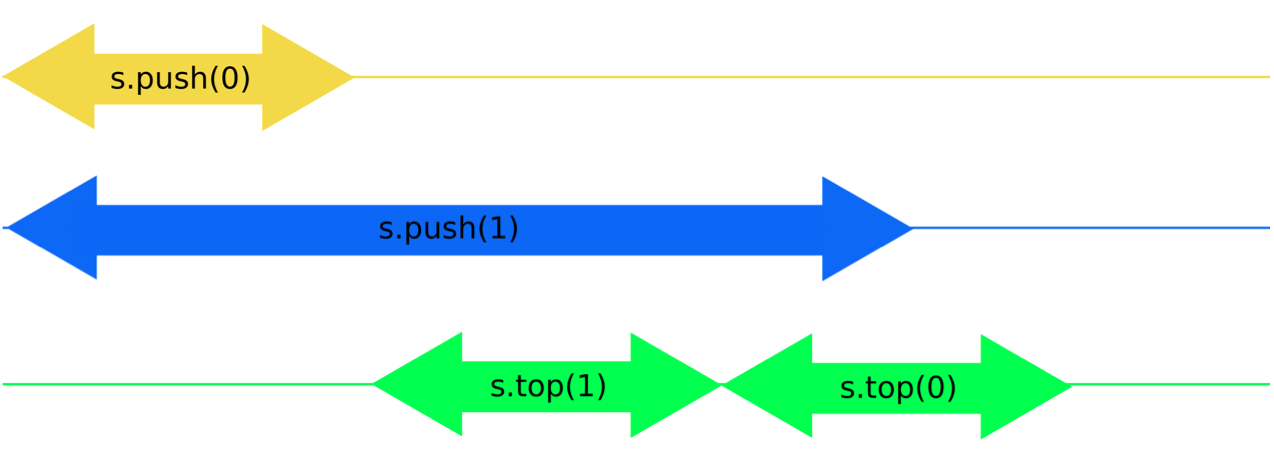
\includegraphics[scale=0.27]{figure1}
    \end{centering}
  }
\end{itemize}

\begin{enumerate}
  \item{\textsl{Indica si la historia es linearizable}}
  \item{\textsl{Indica si la historia es secuencialmente consistente}}
\end{enumerate}

\item{\textsl{
      Considera el siguiente código.\\
      La clase \texttt{AtomicInteger} es un contenedor para un valor
      entero. Esta clase contiene el método \texttt{boolean
        CompareAndSet (int expect, int update)} que compara el valor
      actual del objeto con \texttt{expect}. Si los valores son
      iguales, entonces atómicamente se reemplaza el valor del objeto
      con el valor \texttt{update} y se devuelve \texttt{true}. Si los
      valores no son iguales, el objeto no cambia y se regrsa
      \texttt{false}. La clase también contiene el método \texttt{int
        get()} que regresa el valor actual del objeto.\\
      El código muestra la implementación de una cola FIFO. La cola
      guarda a los elementos en el arreglo \texttt{items}, el cual
      supondremos que tiene capacidad infinita; también contiene dos
      campos de la clase \texttt{AtomicInteger.head} que es el índice
      de la casilla del siguiente elemento a ser eliminado y
      \texttt{tail} que es el índice de la casilla en la que se
      guardará el siguiente elemento.
    }

    \renewcommand{\lstlistingname}{}
\begin{lstlisting}[frame=single]
class IQueue<T> f {
   AtomicInteger head = new AtomicInteger(0);
   AtomicInteger tail = new AtomicInteger(0);
   T[] items = (T[]) new Object[Integer.MAX VALUE];
   
   public void enq(T x){
      int slot;
      do {
         slot = tail.get();
      } while (! tail.compareAndSet(slot, slot + 1));
      items[slot] = x;
   }

   public T deq() throws EmptyException {
      T value;
      int slot;
      do {
         slot = head.get();
         value = items[slot];
         if (value == null) {
            throw new EmptyException();
         }
      } while (! head.compareAndSet(slot, slot + 1));
      return value;
   }
}
\end{lstlisting}
    \textsl{Da un ejemplo que muestre que esta implementación no es
      linearizable.}

  }
}

\item{\textsl {
      En clase se vio como construir registros a partir de
      otros. Describir detalladamente el algoritmo que construye
      registros Multi-Writer Atomic a partir de los registros
      Multi-Reader Atomic. Demostrar de manera intuitiva que el
      algoritmo es correcto.
    }}
\end{enumerate}
\end{document}
